\documentclass[1p]{elsarticle_modified}
%\bibliographystyle{elsarticle-num}

%\usepackage[colorlinks]{hyperref}
%\usepackage{abbrmath_seonhwa} %\Abb, \Ascr, \Acal ,\Abf, \Afrak
\usepackage{amsfonts}
\usepackage{amssymb}
\usepackage{amsmath}
\usepackage{amsthm}
\usepackage{scalefnt}
\usepackage{amsbsy}
\usepackage{kotex}
\usepackage{caption}
\usepackage{subfig}
\usepackage{color}
\usepackage{graphicx}
\usepackage{xcolor} %% white, black, red, green, blue, cyan, magenta, yellow
\usepackage{float}
\usepackage{setspace}
\usepackage{hyperref}

\usepackage{tikz}
\usetikzlibrary{arrows}

\usepackage{multirow}
\usepackage{array} % fixed length table
\usepackage{hhline}

%%%%%%%%%%%%%%%%%%%%%
\makeatletter
\renewcommand*\env@matrix[1][\arraystretch]{%
	\edef\arraystretch{#1}%
	\hskip -\arraycolsep
	\let\@ifnextchar\new@ifnextchar
	\array{*\c@MaxMatrixCols c}}
\makeatother %https://tex.stackexchange.com/questions/14071/how-can-i-increase-the-line-spacing-in-a-matrix
%%%%%%%%%%%%%%%

\usepackage[normalem]{ulem}

\newcommand{\msout}[1]{\ifmmode\text{\sout{\ensuremath{#1}}}\else\sout{#1}\fi}
%SOURCE: \msout is \stkout macro in https://tex.stackexchange.com/questions/20609/strikeout-in-math-mode

\newcommand{\cancel}[1]{
	\ifmmode
	{\color{red}\msout{#1}}
	\else
	{\color{red}\sout{#1}}
	\fi
}

\newcommand{\add}[1]{
	{\color{blue}\uwave{#1}}
}

\newcommand{\replace}[2]{
	\ifmmode
	{\color{red}\msout{#1}}{\color{blue}\uwave{#2}}
	\else
	{\color{red}\sout{#1}}{\color{blue}\uwave{#2}}
	\fi
}

\newcommand{\Sol}{\mathcal{S}} %segment
\newcommand{\D}{D} %diagram
\newcommand{\A}{\mathcal{A}} %arc


%%%%%%%%%%%%%%%%%%%%%%%%%%%%%5 test

\def\sl{\operatorname{\textup{SL}}(2,\Cbb)}
\def\psl{\operatorname{\textup{PSL}}(2,\Cbb)}
\def\quan{\mkern 1mu \triangleright \mkern 1mu}

\theoremstyle{definition}
\newtheorem{thm}{Theorem}[section]
\newtheorem{prop}[thm]{Proposition}
\newtheorem{lem}[thm]{Lemma}
\newtheorem{ques}[thm]{Question}
\newtheorem{cor}[thm]{Corollary}
\newtheorem{defn}[thm]{Definition}
\newtheorem{exam}[thm]{Example}
\newtheorem{rmk}[thm]{Remark}
\newtheorem{alg}[thm]{Algorithm}

\newcommand{\I}{\sqrt{-1}}
\begin{document}

%\begin{frontmatter}
%
%\title{Boundary parabolic representations of knots up to 8 crossings}
%
%%% Group authors per affiliation:
%\author{Yunhi Cho} 
%\address{Department of Mathematics, University of Seoul, Seoul, Korea}
%\ead{yhcho@uos.ac.kr}
%
%
%\author{Seonhwa Kim} %\fnref{s_kim}}
%\address{Center for Geometry and Physics, Institute for Basic Science, Pohang, 37673, Korea}
%\ead{ryeona17@ibs.re.kr}
%
%\author{Hyuk Kim}
%\address{Department of Mathematical Sciences, Seoul National University, Seoul 08826, Korea}
%\ead{hyukkim@snu.ac.kr}
%
%\author{Seokbeom Yoon}
%\address{Department of Mathematical Sciences, Seoul National University, Seoul, 08826,  Korea}
%\ead{sbyoon15@snu.ac.kr}
%
%\begin{abstract}
%We find all boundary parabolic representation of knots up to 8 crossings.
%
%\end{abstract}
%\begin{keyword}
%    \MSC[2010] 57M25 
%\end{keyword}
%
%\end{frontmatter}

%\linenumbers
%\tableofcontents
%
\newcommand\colored[1]{\textcolor{white}{\rule[-0.35ex]{0.8em}{1.4ex}}\kern-0.8em\color{red} #1}%
%\newcommand\colored[1]{\textcolor{white}{ #1}\kern-2.17ex	\textcolor{white}{ #1}\kern-1.81ex	\textcolor{white}{ #1}\kern-2.15ex\color{red}#1	}

{\Large $\underline{12n_{0101}~(K12n_{0101})}$}

\setlength{\tabcolsep}{10pt}
\renewcommand{\arraystretch}{1.6}
\vspace{1cm}\begin{tabular}{m{100pt}>{\centering\arraybackslash}m{274pt}}
\multirow{5}{120pt}{
	\centering
	\includegraphics[width=112pt]{../../../GIT/diagram.site/Diagrams/png/2190_12n_0101.png}\\
\ \ \ A knot diagram\footnotemark}&
\allowdisplaybreaks
\textbf{Linearized knot diagam} \\
\cline{2-2}
 &
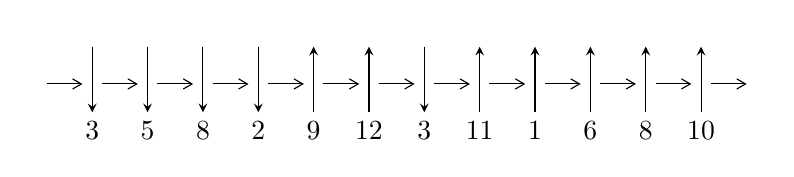
\begin{tikzpicture}[x=20pt, y=17pt]
	% nodes
	\node (C0) at (0, 0) {};
	\node (C1) at (1, 0) {};
	\node (C1U) at (1, +1) {};
	\node (C1D) at (1, -1) {3};

	\node (C2) at (2, 0) {};
	\node (C2U) at (2, +1) {};
	\node (C2D) at (2, -1) {5};

	\node (C3) at (3, 0) {};
	\node (C3U) at (3, +1) {};
	\node (C3D) at (3, -1) {8};

	\node (C4) at (4, 0) {};
	\node (C4U) at (4, +1) {};
	\node (C4D) at (4, -1) {2};

	\node (C5) at (5, 0) {};
	\node (C5U) at (5, +1) {};
	\node (C5D) at (5, -1) {9};

	\node (C6) at (6, 0) {};
	\node (C6U) at (6, +1) {};
	\node (C6D) at (6, -1) {12};

	\node (C7) at (7, 0) {};
	\node (C7U) at (7, +1) {};
	\node (C7D) at (7, -1) {3};

	\node (C8) at (8, 0) {};
	\node (C8U) at (8, +1) {};
	\node (C8D) at (8, -1) {11};

	\node (C9) at (9, 0) {};
	\node (C9U) at (9, +1) {};
	\node (C9D) at (9, -1) {1};

	\node (C10) at (10, 0) {};
	\node (C10U) at (10, +1) {};
	\node (C10D) at (10, -1) {6};

	\node (C11) at (11, 0) {};
	\node (C11U) at (11, +1) {};
	\node (C11D) at (11, -1) {8};

	\node (C12) at (12, 0) {};
	\node (C12U) at (12, +1) {};
	\node (C12D) at (12, -1) {10};
	\node (C13) at (13, 0) {};

	% arrows
	\draw[->,>={angle 60}]
	(C0) edge (C1) (C1) edge (C2) (C2) edge (C3) (C3) edge (C4) (C4) edge (C5) (C5) edge (C6) (C6) edge (C7) (C7) edge (C8) (C8) edge (C9) (C9) edge (C10) (C10) edge (C11) (C11) edge (C12) (C12) edge (C13) ;	\draw[->,>=stealth]
	(C1U) edge (C1D) (C2U) edge (C2D) (C3U) edge (C3D) (C4U) edge (C4D) (C5D) edge (C5U) (C6D) edge (C6U) (C7U) edge (C7D) (C8D) edge (C8U) (C9D) edge (C9U) (C10D) edge (C10U) (C11D) edge (C11U) (C12D) edge (C12U) ;
	\end{tikzpicture} \\
\hhline{~~} \\& 
\textbf{Solving Sequence} \\ \cline{2-2} 
 &
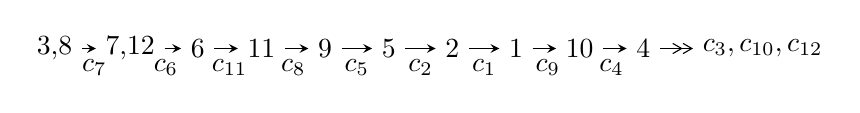
\begin{tikzpicture}[x=23pt, y=7pt]
	% node
	\node (A0) at (-1/8, 0) {3,8};
	\node (A1) at (17/16, 0) {7,12};
	\node (A2) at (17/8, 0) {6};
	\node (A3) at (25/8, 0) {11};
	\node (A4) at (33/8, 0) {9};
	\node (A5) at (41/8, 0) {5};
	\node (A6) at (49/8, 0) {2};
	\node (A7) at (57/8, 0) {1};
	\node (A8) at (65/8, 0) {10};
	\node (A9) at (73/8, 0) {4};
	\node (C1) at (1/2, -1) {$c_{7}$};
	\node (C2) at (13/8, -1) {$c_{6}$};
	\node (C3) at (21/8, -1) {$c_{11}$};
	\node (C4) at (29/8, -1) {$c_{8}$};
	\node (C5) at (37/8, -1) {$c_{5}$};
	\node (C6) at (45/8, -1) {$c_{2}$};
	\node (C7) at (53/8, -1) {$c_{1}$};
	\node (C8) at (61/8, -1) {$c_{9}$};
	\node (C9) at (69/8, -1) {$c_{4}$};
	\node (A10) at (11, 0) {$c_{3},c_{10},c_{12}$};

	% edge
	\draw[->,>=stealth]	
	(A0) edge (A1) (A1) edge (A2) (A2) edge (A3) (A3) edge (A4) (A4) edge (A5) (A5) edge (A6) (A6) edge (A7) (A7) edge (A8) (A8) edge (A9) ;
	\draw[->>,>={angle 60}]	
	(A9) edge (A10);
\end{tikzpicture} \\ 

\end{tabular} \\

\footnotetext{
The image of knot diagram is generated by the software ``\textbf{Draw programme}" developed by Andrew Bartholomew(\url{http://www.layer8.co.uk/maths/draw/index.htm\#Running-draw}), where we modified some parts for our purpose(\url{https://github.com/CATsTAILs/LinksPainter}).
}\phantom \\ \newline 
\centering \textbf{Ideals for irreducible components\footnotemark of $X_{\text{par}}$} 
 
\begin{align*}
I^u_{1}&=\langle 
1.59917\times10^{63} u^{33}-4.04815\times10^{63} u^{32}+\cdots+1.01107\times10^{66} b+7.19589\times10^{65},\\
\phantom{I^u_{1}}&\phantom{= \langle  }2.84744\times10^{64} u^{33}-3.34343\times10^{64} u^{32}+\cdots+1.61772\times10^{67} a-7.28658\times10^{66},\\
\phantom{I^u_{1}}&\phantom{= \langle  }u^{34}-2 u^{33}+\cdots+400 u-128\rangle \\
I^u_{2}&=\langle 
4784545058115 u^{24} a+8814443854630 u^{24}+\cdots-99015474327346 a+74552531293308,\\
\phantom{I^u_{2}}&\phantom{= \langle  }140691453969588 u^{24} a+1943939955417363 u^{24}+\cdots+540597466811832 a+15906220085088582,\\
\phantom{I^u_{2}}&\phantom{= \langle  }u^{25}- u^{24}+\cdots+4 u+4\rangle \\
I^u_{3}&=\langle 
b+1,\;-4 u^2+2 a-2 u-5,\;u^3+u^2+2 u+1\rangle \\
I^u_{4}&=\langle 
2 a u+b+a+u-1,\;a^2-6 a u+10 a-29 u+47,\;u^2- u-1\rangle \\
\\
I^v_{1}&=\langle 
a,\;-20 v^2+13 b+69 v-1,\;4 v^3-13 v^2- v-1\rangle \\
I^v_{2}&=\langle 
a,\;b^2- b v- b+v+1,\;v^2+v+1\rangle \\
\end{align*}
\raggedright * 6 irreducible components of $\dim_{\mathbb{C}}=0$, with total 98 representations.\\
\footnotetext{All coefficients of polynomials are rational numbers. But the coefficients are sometimes approximated in decimal forms when there is not enough margin.}
\newpage
\renewcommand{\arraystretch}{1}
\centering \section*{I. $I^u_{1}= \langle 1.60\times10^{63} u^{33}-4.05\times10^{63} u^{32}+\cdots+1.01\times10^{66} b+7.20\times10^{65},\;2.85\times10^{64} u^{33}-3.34\times10^{64} u^{32}+\cdots+1.62\times10^{67} a-7.29\times10^{66},\;u^{34}-2 u^{33}+\cdots+400 u-128 \rangle$}
\flushleft \textbf{(i) Arc colorings}\\
\begin{tabular}{m{7pt} m{180pt} m{7pt} m{180pt} }
\flushright $a_{3}=$&$\begin{pmatrix}0\\u\end{pmatrix}$ \\
\flushright $a_{8}=$&$\begin{pmatrix}1\\0\end{pmatrix}$ \\
\flushright $a_{7}=$&$\begin{pmatrix}1\\- u^2\end{pmatrix}$ \\
\flushright $a_{12}=$&$\begin{pmatrix}-0.00176016 u^{33}+0.00206675 u^{32}+\cdots+0.145149 u+0.450423\\-0.00158165 u^{33}+0.00400381 u^{32}+\cdots+2.00876 u-0.711707\end{pmatrix}$ \\
\flushright $a_{6}=$&$\begin{pmatrix}-0.000752148 u^{33}+0.00180308 u^{32}+\cdots-0.0951497 u+0.841117\\0.00232746 u^{33}-0.00334332 u^{32}+\cdots+0.699372 u-0.556479\end{pmatrix}$ \\
\flushright $a_{11}=$&$\begin{pmatrix}-0.000178509 u^{33}-0.00193705 u^{32}+\cdots-1.86361 u+1.16213\\-0.00158165 u^{33}+0.00400381 u^{32}+\cdots+2.00876 u-0.711707\end{pmatrix}$ \\
\flushright $a_{9}=$&$\begin{pmatrix}-0.000793255 u^{33}+0.000256525 u^{32}+\cdots+1.90039 u+0.0186257\\-0.00108195 u^{33}+0.00161394 u^{32}+\cdots-1.21132 u+0.797112\end{pmatrix}$ \\
\flushright $a_{5}=$&$\begin{pmatrix}0.00194472 u^{33}-0.00378095 u^{32}+\cdots-4.35824 u+0.981712\\-0.00233421 u^{33}+0.00660539 u^{32}+\cdots+6.08710 u-1.30793\end{pmatrix}$ \\
\flushright $a_{2}=$&$\begin{pmatrix}0.000389490 u^{33}-0.00282444 u^{32}+\cdots-1.72886 u+0.326216\\-0.00233421 u^{33}+0.00660539 u^{32}+\cdots+6.08710 u-1.30793\end{pmatrix}$ \\
\flushright $a_{1}=$&$\begin{pmatrix}0.000389490 u^{33}-0.00282444 u^{32}+\cdots-1.72886 u+0.326216\\-0.00149271 u^{33}+0.00529712 u^{32}+\cdots+5.21906 u-1.04611\end{pmatrix}$ \\
\flushright $a_{10}=$&$\begin{pmatrix}-0.00250395 u^{33}+0.00347839 u^{32}+\cdots+1.84036 u+0.964059\\0.00443973 u^{33}-0.00740068 u^{32}+\cdots-2.07611 u-0.614602\end{pmatrix}$ \\
\flushright $a_{4}=$&$\begin{pmatrix}- u\\u\end{pmatrix}$\\&\end{tabular}
\flushleft \textbf{(ii) Obstruction class $= -1$}\\~\\
\flushleft \textbf{(iii) Cusp Shapes $= -0.0304081 u^{33}+0.0343758 u^{32}+\cdots+21.2214 u+3.74656$}\\~\\
\newpage\renewcommand{\arraystretch}{1}
\flushleft \textbf{(iv) u-Polynomials at the component}\newline \\
\begin{tabular}{m{50pt}|m{274pt}}
Crossings & \hspace{64pt}u-Polynomials at each crossing \\
\hline $$\begin{aligned}c_{1}\end{aligned}$$&$\begin{aligned}
&u^{34}+19 u^{33}+\cdots+24097 u+256
\end{aligned}$\\
\hline $$\begin{aligned}c_{2},c_{4}\end{aligned}$$&$\begin{aligned}
&u^{34}-5 u^{33}+\cdots+129 u+16
\end{aligned}$\\
\hline $$\begin{aligned}c_{3},c_{7}\end{aligned}$$&$\begin{aligned}
&u^{34}-2 u^{33}+\cdots+400 u-128
\end{aligned}$\\
\hline $$\begin{aligned}c_{5},c_{6}\end{aligned}$$&$\begin{aligned}
&8(8 u^{34}-12 u^{33}+\cdots-20 u-4)
\end{aligned}$\\
\hline $$\begin{aligned}c_{8},c_{9},c_{11}\\c_{12}\end{aligned}$$&$\begin{aligned}
&u^{34}-3 u^{33}+\cdots-14 u+1
\end{aligned}$\\
\hline $$\begin{aligned}c_{10}\end{aligned}$$&$\begin{aligned}
&u^{34}+6 u^{33}+\cdots-960 u-256
\end{aligned}$\\
\hline
\end{tabular}\\~\\
\newpage\renewcommand{\arraystretch}{1}
\flushleft \textbf{(v) Riley Polynomials at the component}\newline \\
\begin{tabular}{m{50pt}|m{274pt}}
Crossings & \hspace{64pt}Riley Polynomials at each crossing \\
\hline $$\begin{aligned}c_{1}\end{aligned}$$&$\begin{aligned}
&y^{34}-3 y^{33}+\cdots-473567809 y+65536
\end{aligned}$\\
\hline $$\begin{aligned}c_{2},c_{4}\end{aligned}$$&$\begin{aligned}
&y^{34}-19 y^{33}+\cdots-24097 y+256
\end{aligned}$\\
\hline $$\begin{aligned}c_{3},c_{7}\end{aligned}$$&$\begin{aligned}
&y^{34}+12 y^{33}+\cdots-83200 y+16384
\end{aligned}$\\
\hline $$\begin{aligned}c_{5},c_{6}\end{aligned}$$&$\begin{aligned}
&64(64 y^{34}-336 y^{33}+\cdots-672 y+16)
\end{aligned}$\\
\hline $$\begin{aligned}c_{8},c_{9},c_{11}\\c_{12}\end{aligned}$$&$\begin{aligned}
&y^{34}+15 y^{33}+\cdots-100 y+1
\end{aligned}$\\
\hline $$\begin{aligned}c_{10}\end{aligned}$$&$\begin{aligned}
&y^{34}+22 y^{33}+\cdots-872448 y+65536
\end{aligned}$\\
\hline
\end{tabular}\\~\\
\newpage\flushleft \textbf{(vi) Complex Volumes and Cusp Shapes}
$$\begin{array}{c|c|c}  
\text{Solutions to }I^u_{1}& \I (\text{vol} + \sqrt{-1}CS) & \text{Cusp shape}\\
 \hline 
\begin{aligned}
u &= -0.794712 + 0.456011 I \\
a &= -0.188293 + 1.208770 I \\
b &= -0.240887 - 0.522076 I\end{aligned}
 & -1.49824 + 0.24728 I & \phantom{-}0.14004 - 3.83407 I \\ \hline\begin{aligned}
u &= -0.794712 - 0.456011 I \\
a &= -0.188293 - 1.208770 I \\
b &= -0.240887 + 0.522076 I\end{aligned}
 & -1.49824 - 0.24728 I & \phantom{-}0.14004 + 3.83407 I \\ \hline\begin{aligned}
u &= -0.832178 + 0.785945 I \\
a &= \phantom{-}0.447308 - 0.208329 I \\
b &= -0.408436 + 0.761565 I\end{aligned}
 & -1.67003 - 2.80421 I & \phantom{-}0.86901 + 5.38758 I \\ \hline\begin{aligned}
u &= -0.832178 - 0.785945 I \\
a &= \phantom{-}0.447308 + 0.208329 I \\
b &= -0.408436 - 0.761565 I\end{aligned}
 & -1.67003 + 2.80421 I & \phantom{-}0.86901 - 5.38758 I \\ \hline\begin{aligned}
u &= -0.059447 + 1.230540 I \\
a &= -1.319320 + 0.166847 I \\
b &= -1.210090 + 0.579679 I\end{aligned}
 & \phantom{-}5.21011 - 1.36737 I & \phantom{-}3.81985 - 1.34255 I \\ \hline\begin{aligned}
u &= -0.059447 - 1.230540 I \\
a &= -1.319320 - 0.166847 I \\
b &= -1.210090 - 0.579679 I\end{aligned}
 & \phantom{-}5.21011 + 1.36737 I & \phantom{-}3.81985 + 1.34255 I \\ \hline\begin{aligned}
u &= \phantom{-}0.393005 + 1.221530 I \\
a &= -1.127800 - 0.513887 I \\
b &= -1.39318 - 0.40476 I\end{aligned}
 & \phantom{-}4.28492 - 4.01263 I & -0.30460 + 7.28252 I \\ \hline\begin{aligned}
u &= \phantom{-}0.393005 - 1.221530 I \\
a &= -1.127800 + 0.513887 I \\
b &= -1.39318 + 0.40476 I\end{aligned}
 & \phantom{-}4.28492 + 4.01263 I & -0.30460 - 7.28252 I \\ \hline\begin{aligned}
u &= \phantom{-}0.720618 + 1.080510 I \\
a &= -0.955921 - 0.511219 I \\
b &= -0.583998 + 0.942648 I\end{aligned}
 & \phantom{-}2.44267 - 4.12024 I & \phantom{-}3.28639 + 5.00197 I \\ \hline\begin{aligned}
u &= \phantom{-}0.720618 - 1.080510 I \\
a &= -0.955921 + 0.511219 I \\
b &= -0.583998 - 0.942648 I\end{aligned}
 & \phantom{-}2.44267 + 4.12024 I & \phantom{-}3.28639 - 5.00197 I\\
 \hline 
 \end{array}$$\newpage$$\begin{array}{c|c|c}  
\text{Solutions to }I^u_{1}& \I (\text{vol} + \sqrt{-1}CS) & \text{Cusp shape}\\
 \hline 
\begin{aligned}
u &= \phantom{-}0.650367 + 0.044010 I \\
a &= \phantom{-}1.12796 - 1.09386 I \\
b &= -0.930560 + 0.199538 I\end{aligned}
 & \phantom{-}0.690195 + 0.080524 I & \phantom{-}8.8969 - 15.6686 I \\ \hline\begin{aligned}
u &= \phantom{-}0.650367 - 0.044010 I \\
a &= \phantom{-}1.12796 + 1.09386 I \\
b &= -0.930560 - 0.199538 I\end{aligned}
 & \phantom{-}0.690195 - 0.080524 I & \phantom{-}8.8969 + 15.6686 I \\ \hline\begin{aligned}
u &= \phantom{-}0.39356 + 1.36168 I \\
a &= \phantom{-}1.203780 - 0.501729 I \\
b &= \phantom{-}0.474808 - 1.157210 I\end{aligned}
 & -6.44421 - 6.99411 I & -2.98433 + 6.50573 I \\ \hline\begin{aligned}
u &= \phantom{-}0.39356 - 1.36168 I \\
a &= \phantom{-}1.203780 + 0.501729 I \\
b &= \phantom{-}0.474808 + 1.157210 I\end{aligned}
 & -6.44421 + 6.99411 I & -2.98433 - 6.50573 I \\ \hline\begin{aligned}
u &= -0.87961 + 1.15587 I \\
a &= -0.913426 + 0.382143 I \\
b &= -0.464763 - 1.155720 I\end{aligned}
 & -0.80760 + 9.64229 I & -2.05779 - 8.26691 I \\ \hline\begin{aligned}
u &= -0.87961 - 1.15587 I \\
a &= -0.913426 - 0.382143 I \\
b &= -0.464763 + 1.155720 I\end{aligned}
 & -0.80760 - 9.64229 I & -2.05779 + 8.26691 I \\ \hline\begin{aligned}
u &= \phantom{-}1.35864 + 0.52500 I \\
a &= \phantom{-}0.193842 - 0.210406 I \\
b &= \phantom{-}0.541334 + 1.208100 I\end{aligned}
 & -5.25087 + 10.27080 I & -2.87805 - 7.59115 I \\ \hline\begin{aligned}
u &= \phantom{-}1.35864 - 0.52500 I \\
a &= \phantom{-}0.193842 + 0.210406 I \\
b &= \phantom{-}0.541334 - 1.208100 I\end{aligned}
 & -5.25087 - 10.27080 I & -2.87805 + 7.59115 I \\ \hline\begin{aligned}
u &= -1.45769 + 0.28609 I \\
a &= \phantom{-}0.190522 + 0.239926 I \\
b &= \phantom{-}0.437920 - 1.051280 I\end{aligned}
 & -3.76533 - 4.11043 I & -1.57621 + 5.08065 I \\ \hline\begin{aligned}
u &= -1.45769 - 0.28609 I \\
a &= \phantom{-}0.190522 - 0.239926 I \\
b &= \phantom{-}0.437920 + 1.051280 I\end{aligned}
 & -3.76533 + 4.11043 I & -1.57621 - 5.08065 I\\
 \hline 
 \end{array}$$\newpage$$\begin{array}{c|c|c}  
\text{Solutions to }I^u_{1}& \I (\text{vol} + \sqrt{-1}CS) & \text{Cusp shape}\\
 \hline 
\begin{aligned}
u &= -0.20308 + 1.50476 I \\
a &= \phantom{-}0.650989 - 0.156764 I \\
b &= \phantom{-}0.450406 - 0.473646 I\end{aligned}
 & \phantom{-}3.73592 + 1.81982 I & \phantom{-}0.08831 + 1.82850 I \\ \hline\begin{aligned}
u &= -0.20308 - 1.50476 I \\
a &= \phantom{-}0.650989 + 0.156764 I \\
b &= \phantom{-}0.450406 + 0.473646 I\end{aligned}
 & \phantom{-}3.73592 - 1.81982 I & \phantom{-}0.08831 - 1.82850 I \\ \hline\begin{aligned}
u &= -0.475511\phantom{ +0.000000I} \\
a &= \phantom{-}1.67568\phantom{ +0.000000I} \\
b &= -0.0960916\phantom{ +0.000000I}\end{aligned}
 & -1.21807\phantom{ +0.000000I} & -10.2050\phantom{ +0.000000I} \\ \hline\begin{aligned}
u &= \phantom{-}0.81913 + 1.33067 I \\
a &= \phantom{-}1.41026 + 0.17074 I \\
b &= \phantom{-}0.64527 - 1.33926 I\end{aligned}
 & -2.5846 - 17.9258 I & -1.78648 + 9.71152 I \\ \hline\begin{aligned}
u &= \phantom{-}0.81913 - 1.33067 I \\
a &= \phantom{-}1.41026 - 0.17074 I \\
b &= \phantom{-}0.64527 + 1.33926 I\end{aligned}
 & -2.5846 + 17.9258 I & -1.78648 - 9.71152 I \\ \hline\begin{aligned}
u &= \phantom{-}0.042281 + 0.429124 I \\
a &= \phantom{-}0.167290 - 0.199986 I \\
b &= \phantom{-}0.23202 + 1.50109 I\end{aligned}
 & -10.86120 + 5.07702 I & \phantom{-}13.61431 + 1.23428 I \\ \hline\begin{aligned}
u &= \phantom{-}0.042281 - 0.429124 I \\
a &= \phantom{-}0.167290 + 0.199986 I \\
b &= \phantom{-}0.23202 - 1.50109 I\end{aligned}
 & -10.86120 - 5.07702 I & \phantom{-}13.61431 - 1.23428 I \\ \hline\begin{aligned}
u &= -0.68128 + 1.43732 I \\
a &= \phantom{-}1.280410 + 0.028747 I \\
b &= \phantom{-}0.641425 + 1.240980 I\end{aligned}
 & \phantom{-}0.15639 + 11.56040 I & \phantom{-}0.62674 - 6.67003 I \\ \hline\begin{aligned}
u &= -0.68128 - 1.43732 I \\
a &= \phantom{-}1.280410 - 0.028747 I \\
b &= \phantom{-}0.641425 - 1.240980 I\end{aligned}
 & \phantom{-}0.15639 - 11.56040 I & \phantom{-}0.62674 + 6.67003 I \\ \hline\begin{aligned}
u &= -0.09648 + 1.64631 I \\
a &= \phantom{-}0.710357 + 0.202519 I \\
b &= \phantom{-}0.514600 + 0.733387 I\end{aligned}
 & \phantom{-}3.88573 + 4.85584 I & \phantom{-}1.37960 - 7.57560 I\\
 \hline 
 \end{array}$$\newpage$$\begin{array}{c|c|c}  
\text{Solutions to }I^u_{1}& \I (\text{vol} + \sqrt{-1}CS) & \text{Cusp shape}\\
 \hline 
\begin{aligned}
u &= -0.09648 - 1.64631 I \\
a &= \phantom{-}0.710357 - 0.202519 I \\
b &= \phantom{-}0.514600 - 0.733387 I\end{aligned}
 & \phantom{-}3.88573 - 4.85584 I & \phantom{-}1.37960 + 7.57560 I \\ \hline\begin{aligned}
u &= \phantom{-}0.327433\phantom{ +0.000000I} \\
a &= \phantom{-}1.02586\phantom{ +0.000000I} \\
b &= -0.565142\phantom{ +0.000000I}\end{aligned}
 & \phantom{-}0.885375\phantom{ +0.000000I} & \phantom{-}11.5390\phantom{ +0.000000I} \\ \hline\begin{aligned}
u &= \phantom{-}1.70092 + 0.16271 I \\
a &= \phantom{-}0.068129 - 0.255918 I \\
b &= \phantom{-}0.124754 + 0.960782 I\end{aligned}
 & -12.03160 + 0.52686 I & \phantom{-0.000000 } 0. - 14.5498 I \\ \hline\begin{aligned}
u &= \phantom{-}1.70092 - 0.16271 I \\
a &= \phantom{-}0.068129 + 0.255918 I \\
b &= \phantom{-}0.124754 - 0.960782 I\end{aligned}
 & -12.03160 - 0.52686 I & \phantom{-0.000000 -}0. + 14.5498 I\\
 \hline 
 \end{array}$$\newpage\newpage\renewcommand{\arraystretch}{1}
\centering \section*{II. $I^u_{2}= \langle 4.78\times10^{12} a u^{24}+8.81\times10^{12} u^{24}+\cdots-9.90\times10^{13} a+7.46\times10^{13},\;1.41\times10^{14} a u^{24}+1.94\times10^{15} u^{24}+\cdots+5.41\times10^{14} a+1.59\times10^{16},\;u^{25}- u^{24}+\cdots+4 u+4 \rangle$}
\flushleft \textbf{(i) Arc colorings}\\
\begin{tabular}{m{7pt} m{180pt} m{7pt} m{180pt} }
\flushright $a_{3}=$&$\begin{pmatrix}0\\u\end{pmatrix}$ \\
\flushright $a_{8}=$&$\begin{pmatrix}1\\0\end{pmatrix}$ \\
\flushright $a_{7}=$&$\begin{pmatrix}1\\- u^2\end{pmatrix}$ \\
\flushright $a_{12}=$&$\begin{pmatrix}a\\-0.258951 a u^{24}-0.477058 u^{24}+\cdots+5.35894 a-4.03495\end{pmatrix}$ \\
\flushright $a_{6}=$&$\begin{pmatrix}-0.124665 a u^{24}-3.59160 u^{24}+\cdots+1.27680 a-26.1250\\-0.924644 a u^{24}+1.04931 u^{24}+\cdots+1.62244 a-2.89924\end{pmatrix}$ \\
\flushright $a_{11}=$&$\begin{pmatrix}0.258951 a u^{24}+0.477058 u^{24}+\cdots-4.35894 a+4.03495\\-0.258951 a u^{24}-0.477058 u^{24}+\cdots+5.35894 a-4.03495\end{pmatrix}$ \\
\flushright $a_{9}=$&$\begin{pmatrix}-1.08855 a u^{24}+0.147616 u^{24}+\cdots-0.207055 a-8.18295\\1.26334 a u^{24}-1.09943 u^{24}+\cdots-2.69616 a+4.52566\end{pmatrix}$ \\
\flushright $a_{5}=$&$\begin{pmatrix}-0.663007 u^{24}+0.208677 u^{23}+\cdots-5.67662 u-0.806984\\0.644979 u^{24}-0.740559 u^{23}+\cdots+3.48093 u-1.06790\end{pmatrix}$ \\
\flushright $a_{2}=$&$\begin{pmatrix}0.0180278 u^{24}+0.531881 u^{23}+\cdots+2.19569 u+1.87488\\0.644979 u^{24}-0.740559 u^{23}+\cdots+3.48093 u-1.06790\end{pmatrix}$ \\
\flushright $a_{1}=$&$\begin{pmatrix}0.0180278 u^{24}+0.531881 u^{23}+\cdots+2.19569 u+1.87488\\0.651848 u^{24}-0.230278 u^{23}+\cdots+5.75268 u+1.13174\end{pmatrix}$ \\
\flushright $a_{10}=$&$\begin{pmatrix}-0.477058 a u^{24}+0.192998 u^{24}+\cdots-4.03495 a-6.54862\\1\end{pmatrix}$ \\
\flushright $a_{4}=$&$\begin{pmatrix}- u\\u\end{pmatrix}$\\&\end{tabular}
\flushleft \textbf{(ii) Obstruction class $= -1$}\\~\\
\flushleft \textbf{(iii) Cusp Shapes $= -\frac{6062761600965}{9238337702138} u^{24}-\frac{3225176474347}{9238337702138} u^{23}+\cdots-\frac{61042729884201}{9238337702138} u-\frac{9798007398656}{4619168851069}$}\\~\\
\newpage\renewcommand{\arraystretch}{1}
\flushleft \textbf{(iv) u-Polynomials at the component}\newline \\
\begin{tabular}{m{50pt}|m{274pt}}
Crossings & \hspace{64pt}u-Polynomials at each crossing \\
\hline $$\begin{aligned}c_{1}\end{aligned}$$&$\begin{aligned}
&(u^{25}+11 u^{24}+\cdots-2 u+1)^{2}
\end{aligned}$\\
\hline $$\begin{aligned}c_{2},c_{4}\end{aligned}$$&$\begin{aligned}
&(u^{25}-3 u^{24}+\cdots-4 u+1)^{2}
\end{aligned}$\\
\hline $$\begin{aligned}c_{3},c_{7}\end{aligned}$$&$\begin{aligned}
&(u^{25}- u^{24}+\cdots+4 u+4)^{2}
\end{aligned}$\\
\hline $$\begin{aligned}c_{5},c_{6}\end{aligned}$$&$\begin{aligned}
&u^{50}-4 u^{49}+\cdots+9832 u+2407
\end{aligned}$\\
\hline $$\begin{aligned}c_{8},c_{9},c_{11}\\c_{12}\end{aligned}$$&$\begin{aligned}
&u^{50}+8 u^{49}+\cdots+434 u+49
\end{aligned}$\\
\hline $$\begin{aligned}c_{10}\end{aligned}$$&$\begin{aligned}
&(u^{25}-2 u^{24}+\cdots+3 u-1)^{2}
\end{aligned}$\\
\hline
\end{tabular}\\~\\
\newpage\renewcommand{\arraystretch}{1}
\flushleft \textbf{(v) Riley Polynomials at the component}\newline \\
\begin{tabular}{m{50pt}|m{274pt}}
Crossings & \hspace{64pt}Riley Polynomials at each crossing \\
\hline $$\begin{aligned}c_{1}\end{aligned}$$&$\begin{aligned}
&(y^{25}+9 y^{24}+\cdots-2 y-1)^{2}
\end{aligned}$\\
\hline $$\begin{aligned}c_{2},c_{4}\end{aligned}$$&$\begin{aligned}
&(y^{25}-11 y^{24}+\cdots-2 y-1)^{2}
\end{aligned}$\\
\hline $$\begin{aligned}c_{3},c_{7}\end{aligned}$$&$\begin{aligned}
&(y^{25}+15 y^{24}+\cdots-88 y-16)^{2}
\end{aligned}$\\
\hline $$\begin{aligned}c_{5},c_{6}\end{aligned}$$&$\begin{aligned}
&y^{50}+18 y^{49}+\cdots+211966944 y+5793649
\end{aligned}$\\
\hline $$\begin{aligned}c_{8},c_{9},c_{11}\\c_{12}\end{aligned}$$&$\begin{aligned}
&y^{50}+30 y^{49}+\cdots+4704 y+2401
\end{aligned}$\\
\hline $$\begin{aligned}c_{10}\end{aligned}$$&$\begin{aligned}
&(y^{25}+8 y^{24}+\cdots+11 y-1)^{2}
\end{aligned}$\\
\hline
\end{tabular}\\~\\
\newpage\flushleft \textbf{(vi) Complex Volumes and Cusp Shapes}
$$\begin{array}{c|c|c}  
\text{Solutions to }I^u_{2}& \I (\text{vol} + \sqrt{-1}CS) & \text{Cusp shape}\\
 \hline 
\begin{aligned}
u &= \phantom{-}0.111975 + 0.962557 I \\
a &= \phantom{-}1.72008 - 0.26684 I \\
b &= \phantom{-}0.665176 + 0.113324 I\end{aligned}
 & -3.49154 - 2.66172 I & \phantom{-}1.28523 + 3.57661 I \\ \hline\begin{aligned}
u &= \phantom{-}0.111975 + 0.962557 I \\
a &= -1.13128 + 1.66859 I \\
b &= -0.381710 + 1.094260 I\end{aligned}
 & -3.49154 - 2.66172 I & \phantom{-}1.28523 + 3.57661 I \\ \hline\begin{aligned}
u &= \phantom{-}0.111975 - 0.962557 I \\
a &= \phantom{-}1.72008 + 0.26684 I \\
b &= \phantom{-}0.665176 - 0.113324 I\end{aligned}
 & -3.49154 + 2.66172 I & \phantom{-}1.28523 - 3.57661 I \\ \hline\begin{aligned}
u &= \phantom{-}0.111975 - 0.962557 I \\
a &= -1.13128 - 1.66859 I \\
b &= -0.381710 - 1.094260 I\end{aligned}
 & -3.49154 + 2.66172 I & \phantom{-}1.28523 - 3.57661 I \\ \hline\begin{aligned}
u &= -1.061780 + 0.135314 I \\
a &= \phantom{-}0.240534 + 0.826928 I \\
b &= \phantom{-}0.394082 - 0.313244 I\end{aligned}
 & -1.76494 + 0.43356 I & \phantom{-}0.911962 + 0.045065 I \\ \hline\begin{aligned}
u &= -1.061780 + 0.135314 I \\
a &= \phantom{-}0.157939 + 0.550535 I \\
b &= -0.287348 - 0.868580 I\end{aligned}
 & -1.76494 + 0.43356 I & \phantom{-}0.911962 + 0.045065 I \\ \hline\begin{aligned}
u &= -1.061780 - 0.135314 I \\
a &= \phantom{-}0.240534 - 0.826928 I \\
b &= \phantom{-}0.394082 + 0.313244 I\end{aligned}
 & -1.76494 - 0.43356 I & \phantom{-}0.911962 - 0.045065 I \\ \hline\begin{aligned}
u &= -1.061780 - 0.135314 I \\
a &= \phantom{-}0.157939 - 0.550535 I \\
b &= -0.287348 + 0.868580 I\end{aligned}
 & -1.76494 - 0.43356 I & \phantom{-}0.911962 - 0.045065 I \\ \hline\begin{aligned}
u &= \phantom{-}0.465035 + 1.033020 I \\
a &= \phantom{-}1.48303 - 0.11082 I \\
b &= \phantom{-}0.86062 - 1.16851 I\end{aligned}
 & -5.20581 - 5.41987 I & -3.35697 + 6.54919 I \\ \hline\begin{aligned}
u &= \phantom{-}0.465035 + 1.033020 I \\
a &= \phantom{-}0.034490 + 0.179256 I \\
b &= \phantom{-}0.30041 + 1.61643 I\end{aligned}
 & -5.20581 - 5.41987 I & -3.35697 + 6.54919 I\\
 \hline 
 \end{array}$$\newpage$$\begin{array}{c|c|c}  
\text{Solutions to }I^u_{2}& \I (\text{vol} + \sqrt{-1}CS) & \text{Cusp shape}\\
 \hline 
\begin{aligned}
u &= \phantom{-}0.465035 - 1.033020 I \\
a &= \phantom{-}1.48303 + 0.11082 I \\
b &= \phantom{-}0.86062 + 1.16851 I\end{aligned}
 & -5.20581 + 5.41987 I & -3.35697 - 6.54919 I \\ \hline\begin{aligned}
u &= \phantom{-}0.465035 - 1.033020 I \\
a &= \phantom{-}0.034490 - 0.179256 I \\
b &= \phantom{-}0.30041 - 1.61643 I\end{aligned}
 & -5.20581 + 5.41987 I & -3.35697 - 6.54919 I \\ \hline\begin{aligned}
u &= \phantom{-}1.096160 + 0.296196 I \\
a &= \phantom{-}0.424515 + 0.723296 I \\
b &= \phantom{-}0.877631 - 0.175572 I\end{aligned}
 & -2.14901 + 5.11531 I & -0.18255 - 5.48464 I \\ \hline\begin{aligned}
u &= \phantom{-}1.096160 + 0.296196 I \\
a &= \phantom{-}0.133523 + 0.354909 I \\
b &= -0.531250 - 1.162460 I\end{aligned}
 & -2.14901 + 5.11531 I & -0.18255 - 5.48464 I \\ \hline\begin{aligned}
u &= \phantom{-}1.096160 - 0.296196 I \\
a &= \phantom{-}0.424515 - 0.723296 I \\
b &= \phantom{-}0.877631 + 0.175572 I\end{aligned}
 & -2.14901 - 5.11531 I & -0.18255 + 5.48464 I \\ \hline\begin{aligned}
u &= \phantom{-}1.096160 - 0.296196 I \\
a &= \phantom{-}0.133523 - 0.354909 I \\
b &= -0.531250 + 1.162460 I\end{aligned}
 & -2.14901 - 5.11531 I & -0.18255 + 5.48464 I \\ \hline\begin{aligned}
u &= -0.202658 + 1.122680 I \\
a &= -1.19686 + 1.38943 I \\
b &= -0.194773 - 1.170190 I\end{aligned}
 & -1.18805 + 2.44039 I & \phantom{-}3.83401 - 3.61173 I \\ \hline\begin{aligned}
u &= -0.202658 + 1.122680 I \\
a &= -1.88921 - 0.26546 I \\
b &= -0.315193 + 0.999419 I\end{aligned}
 & -1.18805 + 2.44039 I & \phantom{-}3.83401 - 3.61173 I \\ \hline\begin{aligned}
u &= -0.202658 - 1.122680 I \\
a &= -1.19686 - 1.38943 I \\
b &= -0.194773 + 1.170190 I\end{aligned}
 & -1.18805 - 2.44039 I & \phantom{-}3.83401 + 3.61173 I \\ \hline\begin{aligned}
u &= -0.202658 - 1.122680 I \\
a &= -1.88921 + 0.26546 I \\
b &= -0.315193 - 0.999419 I\end{aligned}
 & -1.18805 - 2.44039 I & \phantom{-}3.83401 + 3.61173 I\\
 \hline 
 \end{array}$$\newpage$$\begin{array}{c|c|c}  
\text{Solutions to }I^u_{2}& \I (\text{vol} + \sqrt{-1}CS) & \text{Cusp shape}\\
 \hline 
\begin{aligned}
u &= \phantom{-}0.641188 + 0.544744 I \\
a &= -0.583198 + 1.057510 I \\
b &= \phantom{-}0.440569 + 1.132290 I\end{aligned}
 & -6.75523 + 1.05922 I & -7.39395 - 0.37058 I \\ \hline\begin{aligned}
u &= \phantom{-}0.641188 + 0.544744 I \\
a &= \phantom{-}3.42198 + 0.62987 I \\
b &= \phantom{-}0.321269 - 1.257010 I\end{aligned}
 & -6.75523 + 1.05922 I & -7.39395 - 0.37058 I \\ \hline\begin{aligned}
u &= \phantom{-}0.641188 - 0.544744 I \\
a &= -0.583198 - 1.057510 I \\
b &= \phantom{-}0.440569 - 1.132290 I\end{aligned}
 & -6.75523 - 1.05922 I & -7.39395 + 0.37058 I \\ \hline\begin{aligned}
u &= \phantom{-}0.641188 - 0.544744 I \\
a &= \phantom{-}3.42198 - 0.62987 I \\
b &= \phantom{-}0.321269 + 1.257010 I\end{aligned}
 & -6.75523 - 1.05922 I & -7.39395 + 0.37058 I \\ \hline\begin{aligned}
u &= \phantom{-}0.082989 + 0.805818 I \\
a &= \phantom{-}1.048640 + 0.674364 I \\
b &= \phantom{-}0.914155 + 0.667714 I\end{aligned}
 & -3.91328 + 1.39976 I & \phantom{-}0.957222 - 0.060617 I \\ \hline\begin{aligned}
u &= \phantom{-}0.082989 + 0.805818 I \\
a &= \phantom{-}0.258734 + 0.032072 I \\
b &= -0.07533 - 1.53307 I\end{aligned}
 & -3.91328 + 1.39976 I & \phantom{-}0.957222 - 0.060617 I \\ \hline\begin{aligned}
u &= \phantom{-}0.082989 - 0.805818 I \\
a &= \phantom{-}1.048640 - 0.674364 I \\
b &= \phantom{-}0.914155 - 0.667714 I\end{aligned}
 & -3.91328 - 1.39976 I & \phantom{-}0.957222 + 0.060617 I \\ \hline\begin{aligned}
u &= \phantom{-}0.082989 - 0.805818 I \\
a &= \phantom{-}0.258734 - 0.032072 I \\
b &= -0.07533 + 1.53307 I\end{aligned}
 & -3.91328 - 1.39976 I & \phantom{-}0.957222 + 0.060617 I \\ \hline\begin{aligned}
u &= -0.340493 + 0.559321 I \\
a &= \phantom{-}0.708209 - 0.192820 I \\
b &= \phantom{-}0.071939 - 1.290900 I\end{aligned}
 & -3.62565 + 1.50728 I & \phantom{-}1.02072 - 4.31266 I \\ \hline\begin{aligned}
u &= -0.340493 + 0.559321 I \\
a &= \phantom{-}1.57740 + 1.43813 I \\
b &= \phantom{-}0.478126 + 0.780931 I\end{aligned}
 & -3.62565 + 1.50728 I & \phantom{-}1.02072 - 4.31266 I\\
 \hline 
 \end{array}$$\newpage$$\begin{array}{c|c|c}  
\text{Solutions to }I^u_{2}& \I (\text{vol} + \sqrt{-1}CS) & \text{Cusp shape}\\
 \hline 
\begin{aligned}
u &= -0.340493 - 0.559321 I \\
a &= \phantom{-}0.708209 + 0.192820 I \\
b &= \phantom{-}0.071939 + 1.290900 I\end{aligned}
 & -3.62565 - 1.50728 I & \phantom{-}1.02072 + 4.31266 I \\ \hline\begin{aligned}
u &= -0.340493 - 0.559321 I \\
a &= \phantom{-}1.57740 - 1.43813 I \\
b &= \phantom{-}0.478126 - 0.780931 I\end{aligned}
 & -3.62565 - 1.50728 I & \phantom{-}1.02072 + 4.31266 I \\ \hline\begin{aligned}
u &= \phantom{-}0.291960 + 1.368920 I \\
a &= \phantom{-}1.040950 + 0.164703 I \\
b &= \phantom{-}0.535319 - 0.817834 I\end{aligned}
 & \phantom{-}3.63887 + 0.59688 I & \phantom{-}4.46758 - 1.80507 I \\ \hline\begin{aligned}
u &= \phantom{-}0.291960 + 1.368920 I \\
a &= -0.439291 - 0.194912 I \\
b &= -0.625618 - 0.508372 I\end{aligned}
 & \phantom{-}3.63887 + 0.59688 I & \phantom{-}4.46758 - 1.80507 I \\ \hline\begin{aligned}
u &= \phantom{-}0.291960 - 1.368920 I \\
a &= \phantom{-}1.040950 - 0.164703 I \\
b &= \phantom{-}0.535319 + 0.817834 I\end{aligned}
 & \phantom{-}3.63887 - 0.59688 I & \phantom{-}4.46758 + 1.80507 I \\ \hline\begin{aligned}
u &= \phantom{-}0.291960 - 1.368920 I \\
a &= -0.439291 + 0.194912 I \\
b &= -0.625618 + 0.508372 I\end{aligned}
 & \phantom{-}3.63887 - 0.59688 I & \phantom{-}4.46758 + 1.80507 I \\ \hline\begin{aligned}
u &= -0.414621 + 1.342760 I \\
a &= \phantom{-}1.111960 - 0.253905 I \\
b &= \phantom{-}1.076060 - 0.322023 I\end{aligned}
 & \phantom{-}3.05811 + 5.44271 I & \phantom{-}3.50171 - 3.51350 I \\ \hline\begin{aligned}
u &= -0.414621 + 1.342760 I \\
a &= -1.225620 - 0.254682 I \\
b &= -0.730267 - 1.190880 I\end{aligned}
 & \phantom{-}3.05811 + 5.44271 I & \phantom{-}3.50171 - 3.51350 I \\ \hline\begin{aligned}
u &= -0.414621 - 1.342760 I \\
a &= \phantom{-}1.111960 + 0.253905 I \\
b &= \phantom{-}1.076060 + 0.322023 I\end{aligned}
 & \phantom{-}3.05811 - 5.44271 I & \phantom{-}3.50171 + 3.51350 I \\ \hline\begin{aligned}
u &= -0.414621 - 1.342760 I \\
a &= -1.225620 + 0.254682 I \\
b &= -0.730267 + 1.190880 I\end{aligned}
 & \phantom{-}3.05811 - 5.44271 I & \phantom{-}3.50171 + 3.51350 I\\
 \hline 
 \end{array}$$\newpage$$\begin{array}{c|c|c}  
\text{Solutions to }I^u_{2}& \I (\text{vol} + \sqrt{-1}CS) & \text{Cusp shape}\\
 \hline 
\begin{aligned}
u &= -0.55118 + 1.32473 I \\
a &= \phantom{-}1.144470 - 0.278607 I \\
b &= \phantom{-}0.393415 + 1.053730 I\end{aligned}
 & \phantom{-}2.03395 + 5.36637 I & \phantom{-}2.46678 - 3.05337 I \\ \hline\begin{aligned}
u &= -0.55118 + 1.32473 I \\
a &= -0.537601 - 0.047197 I \\
b &= -0.643930 + 0.168348 I\end{aligned}
 & \phantom{-}2.03395 + 5.36637 I & \phantom{-}2.46678 - 3.05337 I \\ \hline\begin{aligned}
u &= -0.55118 - 1.32473 I \\
a &= \phantom{-}1.144470 + 0.278607 I \\
b &= \phantom{-}0.393415 - 1.053730 I\end{aligned}
 & \phantom{-}2.03395 - 5.36637 I & \phantom{-}2.46678 + 3.05337 I \\ \hline\begin{aligned}
u &= -0.55118 - 1.32473 I \\
a &= -0.537601 + 0.047197 I \\
b &= -0.643930 - 0.168348 I\end{aligned}
 & \phantom{-}2.03395 - 5.36637 I & \phantom{-}2.46678 + 3.05337 I \\ \hline\begin{aligned}
u &= \phantom{-}0.64072 + 1.29917 I \\
a &= \phantom{-}1.012980 + 0.450455 I \\
b &= \phantom{-}1.221550 + 0.193871 I\end{aligned}
 & \phantom{-}1.04287 - 11.39030 I & \phantom{-}0.71017 + 7.76664 I \\ \hline\begin{aligned}
u &= \phantom{-}0.64072 + 1.29917 I \\
a &= -1.376020 - 0.045093 I \\
b &= -0.73317 + 1.35425 I\end{aligned}
 & \phantom{-}1.04287 - 11.39030 I & \phantom{-}0.71017 + 7.76664 I \\ \hline\begin{aligned}
u &= \phantom{-}0.64072 - 1.29917 I \\
a &= \phantom{-}1.012980 - 0.450455 I \\
b &= \phantom{-}1.221550 - 0.193871 I\end{aligned}
 & \phantom{-}1.04287 + 11.39030 I & \phantom{-}0.71017 - 7.76664 I \\ \hline\begin{aligned}
u &= \phantom{-}0.64072 - 1.29917 I \\
a &= -1.376020 + 0.045093 I \\
b &= -0.73317 - 1.35425 I\end{aligned}
 & \phantom{-}1.04287 + 11.39030 I & \phantom{-}0.71017 - 7.76664 I \\ \hline\begin{aligned}
u &= -0.518583\phantom{ +0.000000I} \\
a &= -15.1403 + 19.4448 I \\
b &= -0.031733 - 1.001510 I\end{aligned}
 & -4.48394\phantom{ +0.000000I} & -4.44380\phantom{ +0.000000I} \\ \hline\begin{aligned}
u &= -0.518583\phantom{ +0.000000I} \\
a &= -15.1403 - 19.4448 I \\
b &= -0.031733 + 1.001510 I\end{aligned}
 & -4.48394\phantom{ +0.000000I} & -4.44380\phantom{ +0.000000I}\\
 \hline 
 \end{array}$$\newpage\newpage\renewcommand{\arraystretch}{1}
\centering \section*{III. $I^u_{3}= \langle b+1,\;-4 u^2+2 a-2 u-5,\;u^3+u^2+2 u+1 \rangle$}
\flushleft \textbf{(i) Arc colorings}\\
\begin{tabular}{m{7pt} m{180pt} m{7pt} m{180pt} }
\flushright $a_{3}=$&$\begin{pmatrix}0\\u\end{pmatrix}$ \\
\flushright $a_{8}=$&$\begin{pmatrix}1\\0\end{pmatrix}$ \\
\flushright $a_{7}=$&$\begin{pmatrix}1\\- u^2\end{pmatrix}$ \\
\flushright $a_{12}=$&$\begin{pmatrix}2 u^2+u+\frac{5}{2}\\-1\end{pmatrix}$ \\
\flushright $a_{6}=$&$\begin{pmatrix}\frac{1}{4} u^2+\frac{1}{2}\\-\frac{1}{2} u^2\end{pmatrix}$ \\
\flushright $a_{11}=$&$\begin{pmatrix}2 u^2+u+\frac{7}{2}\\-1\end{pmatrix}$ \\
\flushright $a_{9}=$&$\begin{pmatrix}2 u^2+u+\frac{9}{2}\\-1\end{pmatrix}$ \\
\flushright $a_{5}=$&$\begin{pmatrix}u^2+1\\- u^2\end{pmatrix}$ \\
\flushright $a_{2}=$&$\begin{pmatrix}-1\\- u^2\end{pmatrix}$ \\
\flushright $a_{1}=$&$\begin{pmatrix}-1\\0\end{pmatrix}$ \\
\flushright $a_{10}=$&$\begin{pmatrix}2 u^2+u+\frac{7}{2}\\-1\end{pmatrix}$ \\
\flushright $a_{4}=$&$\begin{pmatrix}- u\\u\end{pmatrix}$\\&\end{tabular}
\flushleft \textbf{(ii) Obstruction class $= 1$}\\~\\
\flushleft \textbf{(iii) Cusp Shapes $= -\frac{95}{4} u^2-\frac{49}{4} u-\frac{153}{4}$}\\~\\
\newpage\renewcommand{\arraystretch}{1}
\flushleft \textbf{(iv) u-Polynomials at the component}\newline \\
\begin{tabular}{m{50pt}|m{274pt}}
Crossings & \hspace{64pt}u-Polynomials at each crossing \\
\hline $$\begin{aligned}c_{1},c_{3}\end{aligned}$$&$\begin{aligned}
&u^3- u^2+2 u-1
\end{aligned}$\\
\hline $$\begin{aligned}c_{2}\end{aligned}$$&$\begin{aligned}
&u^3+u^2-1
\end{aligned}$\\
\hline $$\begin{aligned}c_{4}\end{aligned}$$&$\begin{aligned}
&u^3- u^2+1
\end{aligned}$\\
\hline $$\begin{aligned}c_{5}\end{aligned}$$&$\begin{aligned}
&8(8 u^3+12 u^2+4 u-1)
\end{aligned}$\\
\hline $$\begin{aligned}c_{6}\end{aligned}$$&$\begin{aligned}
&8(8 u^3-12 u^2+4 u+1)
\end{aligned}$\\
\hline $$\begin{aligned}c_{7}\end{aligned}$$&$\begin{aligned}
&u^3+u^2+2 u+1
\end{aligned}$\\
\hline $$\begin{aligned}c_{8},c_{9}\end{aligned}$$&$\begin{aligned}
&(u+1)^3
\end{aligned}$\\
\hline $$\begin{aligned}c_{10}\end{aligned}$$&$\begin{aligned}
&u^3
\end{aligned}$\\
\hline $$\begin{aligned}c_{11},c_{12}\end{aligned}$$&$\begin{aligned}
&(u-1)^3
\end{aligned}$\\
\hline
\end{tabular}\\~\\
\newpage\renewcommand{\arraystretch}{1}
\flushleft \textbf{(v) Riley Polynomials at the component}\newline \\
\begin{tabular}{m{50pt}|m{274pt}}
Crossings & \hspace{64pt}Riley Polynomials at each crossing \\
\hline $$\begin{aligned}c_{1},c_{3},c_{7}\end{aligned}$$&$\begin{aligned}
&y^3+3 y^2+2 y-1
\end{aligned}$\\
\hline $$\begin{aligned}c_{2},c_{4}\end{aligned}$$&$\begin{aligned}
&y^3- y^2+2 y-1
\end{aligned}$\\
\hline $$\begin{aligned}c_{5},c_{6}\end{aligned}$$&$\begin{aligned}
&64(64 y^3-80 y^2+40 y-1)
\end{aligned}$\\
\hline $$\begin{aligned}c_{8},c_{9},c_{11}\\c_{12}\end{aligned}$$&$\begin{aligned}
&(y-1)^3
\end{aligned}$\\
\hline $$\begin{aligned}c_{10}\end{aligned}$$&$\begin{aligned}
&y^3
\end{aligned}$\\
\hline
\end{tabular}\\~\\
\newpage\flushleft \textbf{(vi) Complex Volumes and Cusp Shapes}
$$\begin{array}{c|c|c}  
\text{Solutions to }I^u_{3}& \I (\text{vol} + \sqrt{-1}CS) & \text{Cusp shape}\\
 \hline 
\begin{aligned}
u &= -0.215080 + 1.307140 I \\
a &= -1.039800 + 0.182582 I \\
b &= -1.00000\phantom{ +0.000000I}\end{aligned}
 & \phantom{-}4.66906 + 2.82812 I & \phantom{-}3.86575 - 2.65834 I \\ \hline\begin{aligned}
u &= -0.215080 - 1.307140 I \\
a &= -1.039800 - 0.182582 I \\
b &= -1.00000\phantom{ +0.000000I}\end{aligned}
 & \phantom{-}4.66906 - 2.82812 I & \phantom{-}3.86575 + 2.65834 I \\ \hline\begin{aligned}
u &= -0.569840\phantom{ +0.000000I} \\
a &= \phantom{-}2.57960\phantom{ +0.000000I} \\
b &= -1.00000\phantom{ +0.000000I}\end{aligned}
 & \phantom{-}0.531480\phantom{ +0.000000I} & -38.9820\phantom{ +0.000000I}\\
 \hline 
 \end{array}$$\newpage\newpage\renewcommand{\arraystretch}{1}
\centering \section*{IV. $I^u_{4}= \langle 2 a u+b+a+u-1,\;a^2-6 a u+10 a-29 u+47,\;u^2- u-1 \rangle$}
\flushleft \textbf{(i) Arc colorings}\\
\begin{tabular}{m{7pt} m{180pt} m{7pt} m{180pt} }
\flushright $a_{3}=$&$\begin{pmatrix}0\\u\end{pmatrix}$ \\
\flushright $a_{8}=$&$\begin{pmatrix}1\\0\end{pmatrix}$ \\
\flushright $a_{7}=$&$\begin{pmatrix}1\\- u-1\end{pmatrix}$ \\
\flushright $a_{12}=$&$\begin{pmatrix}a\\-2 a u- a- u+1\end{pmatrix}$ \\
\flushright $a_{6}=$&$\begin{pmatrix}3 a u-5 a+18 u-28\\a u+2 u-6\end{pmatrix}$ \\
\flushright $a_{11}=$&$\begin{pmatrix}2 a u+2 a+u-1\\-2 a u- a- u+1\end{pmatrix}$ \\
\flushright $a_{9}=$&$\begin{pmatrix}- a u+a-7 u+11\\1\end{pmatrix}$ \\
\flushright $a_{5}=$&$\begin{pmatrix}1\\- u-1\end{pmatrix}$ \\
\flushright $a_{2}=$&$\begin{pmatrix}u\\- u-1\end{pmatrix}$ \\
\flushright $a_{1}=$&$\begin{pmatrix}u\\-3 u-2\end{pmatrix}$ \\
\flushright $a_{10}=$&$\begin{pmatrix}-4 a u- a-7 u+10\\13 a u+8 a+2 u+2\end{pmatrix}$ \\
\flushright $a_{4}=$&$\begin{pmatrix}- u\\u\end{pmatrix}$\\&\end{tabular}
\flushleft \textbf{(ii) Obstruction class $= 1$}\\~\\
\flushleft \textbf{(iii) Cusp Shapes $= -8$}\\~\\
\newpage\renewcommand{\arraystretch}{1}
\flushleft \textbf{(iv) u-Polynomials at the component}\newline \\
\begin{tabular}{m{50pt}|m{274pt}}
Crossings & \hspace{64pt}u-Polynomials at each crossing \\
\hline $$\begin{aligned}c_{1}\end{aligned}$$&$\begin{aligned}
&(u^2-3 u+1)^2
\end{aligned}$\\
\hline $$\begin{aligned}c_{2},c_{3}\end{aligned}$$&$\begin{aligned}
&(u^2+u-1)^2
\end{aligned}$\\
\hline $$\begin{aligned}c_{4},c_{7}\end{aligned}$$&$\begin{aligned}
&(u^2- u-1)^2
\end{aligned}$\\
\hline $$\begin{aligned}c_{5}\end{aligned}$$&$\begin{aligned}
&u^4-6 u^3+18 u^2-12 u+4
\end{aligned}$\\
\hline $$\begin{aligned}c_{6}\end{aligned}$$&$\begin{aligned}
&u^4+6 u^3+18 u^2+12 u+4
\end{aligned}$\\
\hline $$\begin{aligned}c_{8},c_{9},c_{11}\\c_{12}\end{aligned}$$&$\begin{aligned}
&(u^2+1)^2
\end{aligned}$\\
\hline $$\begin{aligned}c_{10}\end{aligned}$$&$\begin{aligned}
&u^4+7 u^2+1
\end{aligned}$\\
\hline
\end{tabular}\\~\\
\newpage\renewcommand{\arraystretch}{1}
\flushleft \textbf{(v) Riley Polynomials at the component}\newline \\
\begin{tabular}{m{50pt}|m{274pt}}
Crossings & \hspace{64pt}Riley Polynomials at each crossing \\
\hline $$\begin{aligned}c_{1}\end{aligned}$$&$\begin{aligned}
&(y^2-7 y+1)^2
\end{aligned}$\\
\hline $$\begin{aligned}c_{2},c_{3},c_{4}\\c_{7}\end{aligned}$$&$\begin{aligned}
&(y^2-3 y+1)^2
\end{aligned}$\\
\hline $$\begin{aligned}c_{5},c_{6}\end{aligned}$$&$\begin{aligned}
&y^4+188 y^2+16
\end{aligned}$\\
\hline $$\begin{aligned}c_{8},c_{9},c_{11}\\c_{12}\end{aligned}$$&$\begin{aligned}
&(y+1)^4
\end{aligned}$\\
\hline $$\begin{aligned}c_{10}\end{aligned}$$&$\begin{aligned}
&(y^2+7 y+1)^2
\end{aligned}$\\
\hline
\end{tabular}\\~\\
\newpage\flushleft \textbf{(vi) Complex Volumes and Cusp Shapes}
$$\begin{array}{c|c|c}  
\text{Solutions to }I^u_{4}& \I (\text{vol} + \sqrt{-1}CS) & \text{Cusp shape}\\
 \hline 
\begin{aligned}
u &= -0.618034\phantom{ +0.000000I} \\
a &= -6.85410 + 4.23607 I \\
b &= \phantom{-0.000000 -}1.000000 I\end{aligned}
 & -4.27683\phantom{ +0.000000I} & -8.00000\phantom{ +0.000000I} \\ \hline\begin{aligned}
u &= -0.618034\phantom{ +0.000000I} \\
a &= -6.85410 - 4.23607 I \\
b &= \phantom{-0.000000 } -1.000000 I\end{aligned}
 & -4.27683\phantom{ +0.000000I} & -8.00000\phantom{ +0.000000I} \\ \hline\begin{aligned}
u &= \phantom{-}1.61803\phantom{ +0.000000I} \\
a &= -0.145898 + 0.236068 I \\
b &= \phantom{-0.000000 } -1.000000 I\end{aligned}
 & -12.1725\phantom{ +0.000000I} & -8.00000\phantom{ +0.000000I} \\ \hline\begin{aligned}
u &= \phantom{-}1.61803\phantom{ +0.000000I} \\
a &= -0.145898 - 0.236068 I \\
b &= \phantom{-0.000000 -}1.000000 I\end{aligned}
 & -12.1725\phantom{ +0.000000I} & -8.00000\phantom{ +0.000000I}\\
 \hline 
 \end{array}$$\newpage\newpage\renewcommand{\arraystretch}{1}
\centering \section*{V. $I^v_{1}= \langle a,\;-20 v^2+13 b+69 v-1,\;4 v^3-13 v^2- v-1 \rangle$}
\flushleft \textbf{(i) Arc colorings}\\
\begin{tabular}{m{7pt} m{180pt} m{7pt} m{180pt} }
\flushright $a_{3}=$&$\begin{pmatrix}v\\0\end{pmatrix}$ \\
\flushright $a_{8}=$&$\begin{pmatrix}1\\0\end{pmatrix}$ \\
\flushright $a_{7}=$&$\begin{pmatrix}1\\0\end{pmatrix}$ \\
\flushright $a_{12}=$&$\begin{pmatrix}0\\\frac{20}{13} v^2-\frac{69}{13} v+\frac{1}{13}\end{pmatrix}$ \\
\flushright $a_{6}=$&$\begin{pmatrix}1\\\frac{12}{13} v^2-\frac{31}{13} v-\frac{28}{13}\end{pmatrix}$ \\
\flushright $a_{11}=$&$\begin{pmatrix}-\frac{20}{13} v^2+\frac{69}{13} v-\frac{1}{13}\\\frac{20}{13} v^2-\frac{69}{13} v+\frac{1}{13}\end{pmatrix}$ \\
\flushright $a_{9}=$&$\begin{pmatrix}\frac{12}{13} v^2-\frac{31}{13} v-\frac{15}{13}\\-\frac{12}{13} v^2+\frac{31}{13} v+\frac{28}{13}\end{pmatrix}$ \\
\flushright $a_{5}=$&$\begin{pmatrix}-\frac{20}{13} v^2+\frac{69}{13} v-\frac{1}{13}\\4 v^2-13 v-1\end{pmatrix}$ \\
\flushright $a_{2}=$&$\begin{pmatrix}\frac{20}{13} v^2-\frac{56}{13} v+\frac{1}{13}\\-4 v^2+13 v+1\end{pmatrix}$ \\
\flushright $a_{1}=$&$\begin{pmatrix}\frac{20}{13} v^2-\frac{69}{13} v+\frac{1}{13}\\-4 v^2+13 v+1\end{pmatrix}$ \\
\flushright $a_{10}=$&$\begin{pmatrix}1\\-\frac{8}{13} v^2+\frac{38}{13} v-\frac{42}{13}\end{pmatrix}$ \\
\flushright $a_{4}=$&$\begin{pmatrix}v\\0\end{pmatrix}$\\&\end{tabular}
\flushleft \textbf{(ii) Obstruction class $= 1$}\\~\\
\flushleft \textbf{(iii) Cusp Shapes $= -\frac{71}{13} v^2+\frac{373}{13} v-\frac{246}{13}$}\\~\\
\newpage\renewcommand{\arraystretch}{1}
\flushleft \textbf{(iv) u-Polynomials at the component}\newline \\
\begin{tabular}{m{50pt}|m{274pt}}
Crossings & \hspace{64pt}u-Polynomials at each crossing \\
\hline $$\begin{aligned}c_{1},c_{2}\end{aligned}$$&$\begin{aligned}
&(u-1)^3
\end{aligned}$\\
\hline $$\begin{aligned}c_{3},c_{7}\end{aligned}$$&$\begin{aligned}
&u^3
\end{aligned}$\\
\hline $$\begin{aligned}c_{4}\end{aligned}$$&$\begin{aligned}
&(u+1)^3
\end{aligned}$\\
\hline $$\begin{aligned}c_{5},c_{6},c_{8}\\c_{9}\end{aligned}$$&$\begin{aligned}
&u^3+2 u+1
\end{aligned}$\\
\hline $$\begin{aligned}c_{10}\end{aligned}$$&$\begin{aligned}
&u^3-3 u^2+5 u-2
\end{aligned}$\\
\hline $$\begin{aligned}c_{11},c_{12}\end{aligned}$$&$\begin{aligned}
&u^3+2 u-1
\end{aligned}$\\
\hline
\end{tabular}\\~\\
\newpage\renewcommand{\arraystretch}{1}
\flushleft \textbf{(v) Riley Polynomials at the component}\newline \\
\begin{tabular}{m{50pt}|m{274pt}}
Crossings & \hspace{64pt}Riley Polynomials at each crossing \\
\hline $$\begin{aligned}c_{1},c_{2},c_{4}\end{aligned}$$&$\begin{aligned}
&(y-1)^3
\end{aligned}$\\
\hline $$\begin{aligned}c_{3},c_{7}\end{aligned}$$&$\begin{aligned}
&y^3
\end{aligned}$\\
\hline $$\begin{aligned}c_{5},c_{6},c_{8}\\c_{9},c_{11},c_{12}\end{aligned}$$&$\begin{aligned}
&y^3+4 y^2+4 y-1
\end{aligned}$\\
\hline $$\begin{aligned}c_{10}\end{aligned}$$&$\begin{aligned}
&y^3+y^2+13 y-4
\end{aligned}$\\
\hline
\end{tabular}\\~\\
\newpage\flushleft \textbf{(vi) Complex Volumes and Cusp Shapes}
$$\begin{array}{c|c|c}  
\text{Solutions to }I^v_{1}& \I (\text{vol} + \sqrt{-1}CS) & \text{Cusp shape}\\
 \hline 
\begin{aligned}
v &= -0.048505 + 0.268962 I \\
a &= \phantom{-0.000000 } 0 \\
b &= \phantom{-}0.22670 - 1.46771 I\end{aligned}
 & -11.08570 - 5.13794 I & -19.9326 + 7.8597 I \\ \hline\begin{aligned}
v &= -0.048505 - 0.268962 I \\
a &= \phantom{-0.000000 } 0 \\
b &= \phantom{-}0.22670 + 1.46771 I\end{aligned}
 & -11.08570 + 5.13794 I & -19.9326 - 7.8597 I \\ \hline\begin{aligned}
v &= \phantom{-}3.34701\phantom{ +0.000000I} \\
a &= \phantom{-0.000000 } 0 \\
b &= -0.453398\phantom{ +0.000000I}\end{aligned}
 & -0.857735\phantom{ +0.000000I} & \phantom{-}15.9280\phantom{ +0.000000I}\\
 \hline 
 \end{array}$$\newpage\newpage\renewcommand{\arraystretch}{1}
\centering \section*{VI. $I^v_{2}= \langle a,\;b^2- b v- b+v+1,\;v^2+v+1 \rangle$}
\flushleft \textbf{(i) Arc colorings}\\
\begin{tabular}{m{7pt} m{180pt} m{7pt} m{180pt} }
\flushright $a_{3}=$&$\begin{pmatrix}v\\0\end{pmatrix}$ \\
\flushright $a_{8}=$&$\begin{pmatrix}1\\0\end{pmatrix}$ \\
\flushright $a_{7}=$&$\begin{pmatrix}1\\0\end{pmatrix}$ \\
\flushright $a_{12}=$&$\begin{pmatrix}0\\b\end{pmatrix}$ \\
\flushright $a_{6}=$&$\begin{pmatrix}1\\b v+b- v-1\end{pmatrix}$ \\
\flushright $a_{11}=$&$\begin{pmatrix}- b\\b\end{pmatrix}$ \\
\flushright $a_{9}=$&$\begin{pmatrix}b v+b- v\\- b v- b+v+1\end{pmatrix}$ \\
\flushright $a_{5}=$&$\begin{pmatrix}b v+v+2\\- v-1\end{pmatrix}$ \\
\flushright $a_{2}=$&$\begin{pmatrix}- b v-2\\v+1\end{pmatrix}$ \\
\flushright $a_{1}=$&$\begin{pmatrix}- b v- v-2\\v+1\end{pmatrix}$ \\
\flushright $a_{10}=$&$\begin{pmatrix}- b+v\\1\end{pmatrix}$ \\
\flushright $a_{4}=$&$\begin{pmatrix}v\\0\end{pmatrix}$\\&\end{tabular}
\flushleft \textbf{(ii) Obstruction class $= 1$}\\~\\
\flushleft \textbf{(iii) Cusp Shapes $= 4 v-3$}\\~\\
\newpage\renewcommand{\arraystretch}{1}
\flushleft \textbf{(iv) u-Polynomials at the component}\newline \\
\begin{tabular}{m{50pt}|m{274pt}}
Crossings & \hspace{64pt}u-Polynomials at each crossing \\
\hline $$\begin{aligned}c_{1},c_{2}\end{aligned}$$&$\begin{aligned}
&(u-1)^4
\end{aligned}$\\
\hline $$\begin{aligned}c_{3},c_{7}\end{aligned}$$&$\begin{aligned}
&u^4
\end{aligned}$\\
\hline $$\begin{aligned}c_{4}\end{aligned}$$&$\begin{aligned}
&(u+1)^4
\end{aligned}$\\
\hline $$\begin{aligned}c_{5},c_{6},c_{8}\\c_{9}\end{aligned}$$&$\begin{aligned}
&u^4- u^3+2 u^2-2 u+1
\end{aligned}$\\
\hline $$\begin{aligned}c_{10}\end{aligned}$$&$\begin{aligned}
&(u^2+u+1)^2
\end{aligned}$\\
\hline $$\begin{aligned}c_{11},c_{12}\end{aligned}$$&$\begin{aligned}
&u^4+u^3+2 u^2+2 u+1
\end{aligned}$\\
\hline
\end{tabular}\\~\\
\newpage\renewcommand{\arraystretch}{1}
\flushleft \textbf{(v) Riley Polynomials at the component}\newline \\
\begin{tabular}{m{50pt}|m{274pt}}
Crossings & \hspace{64pt}Riley Polynomials at each crossing \\
\hline $$\begin{aligned}c_{1},c_{2},c_{4}\end{aligned}$$&$\begin{aligned}
&(y-1)^4
\end{aligned}$\\
\hline $$\begin{aligned}c_{3},c_{7}\end{aligned}$$&$\begin{aligned}
&y^4
\end{aligned}$\\
\hline $$\begin{aligned}c_{5},c_{6},c_{8}\\c_{9},c_{11},c_{12}\end{aligned}$$&$\begin{aligned}
&y^4+3 y^3+2 y^2+1
\end{aligned}$\\
\hline $$\begin{aligned}c_{10}\end{aligned}$$&$\begin{aligned}
&(y^2+y+1)^2
\end{aligned}$\\
\hline
\end{tabular}\\~\\
\newpage\flushleft \textbf{(vi) Complex Volumes and Cusp Shapes}
$$\begin{array}{c|c|c}  
\text{Solutions to }I^v_{2}& \I (\text{vol} + \sqrt{-1}CS) & \text{Cusp shape}\\
 \hline 
\begin{aligned}
v &= -0.500000 + 0.866025 I \\
a &= \phantom{-0.000000 } 0 \\
b &= \phantom{-}0.621744 - 0.440597 I\end{aligned}
 & -4.93480 - 2.02988 I & -5.00000 + 3.46410 I \\ \hline\begin{aligned}
v &= -0.500000 + 0.866025 I \\
a &= \phantom{-0.000000 } 0 \\
b &= -0.121744 + 1.306620 I\end{aligned}
 & -4.93480 - 2.02988 I & -5.00000 + 3.46410 I \\ \hline\begin{aligned}
v &= -0.500000 - 0.866025 I \\
a &= \phantom{-0.000000 } 0 \\
b &= \phantom{-}0.621744 + 0.440597 I\end{aligned}
 & -4.93480 + 2.02988 I & -5.00000 - 3.46410 I \\ \hline\begin{aligned}
v &= -0.500000 - 0.866025 I \\
a &= \phantom{-0.000000 } 0 \\
b &= -0.121744 - 1.306620 I\end{aligned}
 & -4.93480 + 2.02988 I & -5.00000 - 3.46410 I\\
 \hline 
 \end{array}$$\newpage
\newpage\renewcommand{\arraystretch}{1}
\centering \section*{ VII. u-Polynomials}
\begin{tabular}{m{50pt}|m{274pt}}
Crossings & \hspace{64pt}u-Polynomials at each crossing \\
\hline $$\begin{aligned}c_{1}\end{aligned}$$&$\begin{aligned}
&(u-1)^7(u^2-3 u+1)^2(u^3- u^2+2 u-1)\\
&\cdot((u^{25}+11 u^{24}+\cdots-2 u+1)^{2})(u^{34}+19 u^{33}+\cdots+24097 u+256)
\end{aligned}$\\
\hline $$\begin{aligned}c_{2}\end{aligned}$$&$\begin{aligned}
&((u-1)^7)(u^2+u-1)^2(u^3+u^2-1)(u^{25}-3 u^{24}+\cdots-4 u+1)^{2}\\
&\cdot(u^{34}-5 u^{33}+\cdots+129 u+16)
\end{aligned}$\\
\hline $$\begin{aligned}c_{3}\end{aligned}$$&$\begin{aligned}
&u^7(u^2+u-1)^2(u^3- u^2+2 u-1)(u^{25}- u^{24}+\cdots+4 u+4)^{2}\\
&\cdot(u^{34}-2 u^{33}+\cdots+400 u-128)
\end{aligned}$\\
\hline $$\begin{aligned}c_{4}\end{aligned}$$&$\begin{aligned}
&((u+1)^7)(u^2- u-1)^2(u^3- u^2+1)(u^{25}-3 u^{24}+\cdots-4 u+1)^{2}\\
&\cdot(u^{34}-5 u^{33}+\cdots+129 u+16)
\end{aligned}$\\
\hline $$\begin{aligned}c_{5}\end{aligned}$$&$\begin{aligned}
&64(u^3+2 u+1)(8 u^{3}+12 u^{2}+4 u-1)(u^{4}-6 u^{3}+\cdots-12 u+4)\\
&\cdot(u^4- u^3+2 u^2-2 u+1)(8 u^{34}-12 u^{33}+\cdots-20 u-4)\\
&\cdot(u^{50}-4 u^{49}+\cdots+9832 u+2407)
\end{aligned}$\\
\hline $$\begin{aligned}c_{6}\end{aligned}$$&$\begin{aligned}
&64(u^3+2 u+1)(8 u^3-12 u^2+4 u+1)(u^4- u^3+2 u^2-2 u+1)\\
&\cdot(u^4+6 u^3+18 u^2+12 u+4)(8 u^{34}-12 u^{33}+\cdots-20 u-4)\\
&\cdot(u^{50}-4 u^{49}+\cdots+9832 u+2407)
\end{aligned}$\\
\hline $$\begin{aligned}c_{7}\end{aligned}$$&$\begin{aligned}
&u^7(u^2- u-1)^2(u^3+u^2+2 u+1)(u^{25}- u^{24}+\cdots+4 u+4)^{2}\\
&\cdot(u^{34}-2 u^{33}+\cdots+400 u-128)
\end{aligned}$\\
\hline $$\begin{aligned}c_{8},c_{9}\end{aligned}$$&$\begin{aligned}
&(u+1)^3(u^2+1)^2(u^3+2 u+1)(u^4- u^3+2 u^2-2 u+1)\\
&\cdot(u^{34}-3 u^{33}+\cdots-14 u+1)(u^{50}+8 u^{49}+\cdots+434 u+49)
\end{aligned}$\\
\hline $$\begin{aligned}c_{10}\end{aligned}$$&$\begin{aligned}
&u^3(u^2+u+1)^2(u^3-3 u^2+5 u-2)(u^4+7 u^2+1)\\
&\cdot((u^{25}-2 u^{24}+\cdots+3 u-1)^{2})(u^{34}+6 u^{33}+\cdots-960 u-256)
\end{aligned}$\\
\hline $$\begin{aligned}c_{11},c_{12}\end{aligned}$$&$\begin{aligned}
&(u-1)^3(u^2+1)^2(u^3+2 u-1)(u^4+u^3+2 u^2+2 u+1)\\
&\cdot(u^{34}-3 u^{33}+\cdots-14 u+1)(u^{50}+8 u^{49}+\cdots+434 u+49)
\end{aligned}$\\
\hline
\end{tabular}\newpage\renewcommand{\arraystretch}{1}
\centering \section*{ VIII. Riley Polynomials}
\begin{tabular}{m{50pt}|m{274pt}}
Crossings & \hspace{64pt}Riley Polynomials at each crossing \\
\hline $$\begin{aligned}c_{1}\end{aligned}$$&$\begin{aligned}
&(y-1)^7(y^2-7 y+1)^2(y^3+3 y^2+2 y-1)\\
&\cdot(y^{25}+9 y^{24}+\cdots-2 y-1)^{2}\\
&\cdot(y^{34}-3 y^{33}+\cdots-473567809 y+65536)
\end{aligned}$\\
\hline $$\begin{aligned}c_{2},c_{4}\end{aligned}$$&$\begin{aligned}
&(y-1)^7(y^2-3 y+1)^2(y^3- y^2+2 y-1)\\
&\cdot((y^{25}-11 y^{24}+\cdots-2 y-1)^{2})(y^{34}-19 y^{33}+\cdots-24097 y+256)
\end{aligned}$\\
\hline $$\begin{aligned}c_{3},c_{7}\end{aligned}$$&$\begin{aligned}
&y^7(y^2-3 y+1)^2(y^{3}+3 y^{2}+2 y-1)(y^{25}+15 y^{24}+\cdots-88 y-16)^{2}\\
&\cdot(y^{34}+12 y^{33}+\cdots-83200 y+16384)
\end{aligned}$\\
\hline $$\begin{aligned}c_{5},c_{6}\end{aligned}$$&$\begin{aligned}
&4096(y^{3}+4 y^{2}+4 y-1)(64 y^{3}-80 y^{2}+40 y-1)(y^4+188 y^2+16)\\
&\cdot(y^4+3 y^3+2 y^2+1)(64 y^{34}-336 y^{33}+\cdots-672 y+16)\\
&\cdot(y^{50}+18 y^{49}+\cdots+211966944 y+5793649)
\end{aligned}$\\
\hline $$\begin{aligned}c_{8},c_{9},c_{11}\\c_{12}\end{aligned}$$&$\begin{aligned}
&(y-1)^3(y+1)^4(y^3+4 y^2+4 y-1)(y^4+3 y^3+2 y^2+1)\\
&\cdot(y^{34}+15 y^{33}+\cdots-100 y+1)(y^{50}+30 y^{49}+\cdots+4704 y+2401)
\end{aligned}$\\
\hline $$\begin{aligned}c_{10}\end{aligned}$$&$\begin{aligned}
&y^3(y^2+y+1)^2(y^2+7 y+1)^2(y^3+y^2+13 y-4)\\
&\cdot((y^{25}+8 y^{24}+\cdots+11 y-1)^{2})(y^{34}+22 y^{33}+\cdots-872448 y+65536)
\end{aligned}$\\
\hline
\end{tabular}
\vskip 2pc
\end{document}